
\section{Flowchart}
A flowchart is a type of diagram that represents an algorithm, work flow or process, showing the steps as boxes of various kinds, and their order by connecting them with arrows. 
Flowcharts are used in designing and documenting simple processes or programs. Like other types of diagrams, they help visualize what is going on and thereby help understand a process, and perhaps also find flaws, bottlenecks, and other less-obvious features within it. There are many different types of flowcharts, and each type has its own repertoire of boxes and notational conventions. The two most common types of boxes in a flowchart are:\\
Following is flowchart of system showing flow of control and Data in the software-:

\begin{figure}[h!]
\centering 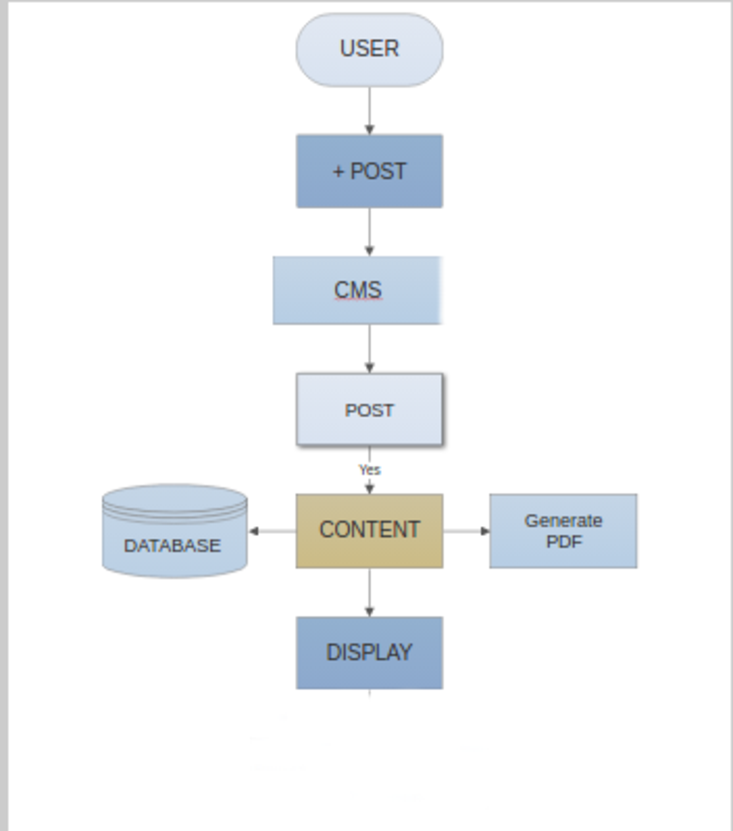
\includegraphics[scale=0.8]{input/images/fc.pdf}
\caption{ Flow diagram}
\label{fig:UI1}
\end{figure}


